\documentclass{standalone}
\usepackage{tikz}
\usetikzlibrary{arrows.meta}
\renewcommand{\familydefault}{\sfdefault} % Sans serif

\tikzset{
	partial ellipse/.style args={#1:#2:#3}{
		insert path={+ (#1:#3) arc (#1:#2:#3)}
	}
}

\begin{document}	
	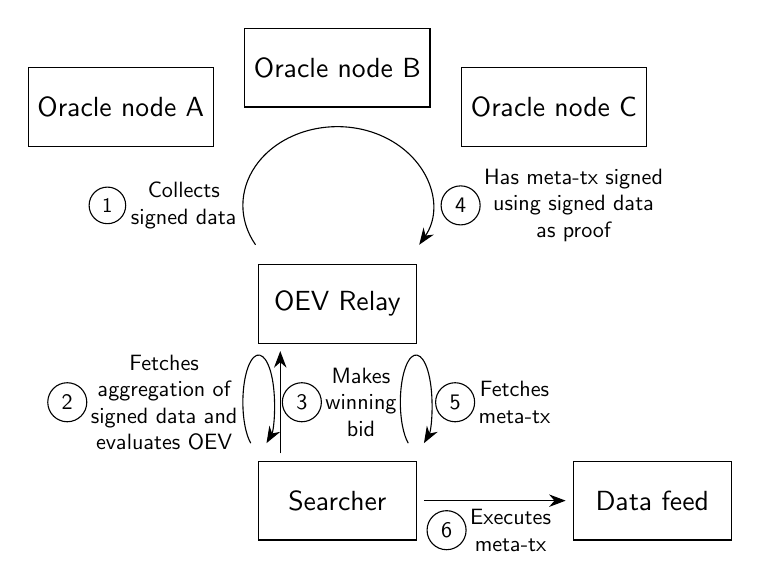
\begin{tikzpicture}
	\node[draw, minimum width=2cm,minimum height=1cm, align=center] at (0,0) (oracle-nodes) {OEV Relay};
	\node[draw, minimum width=2cm,minimum height=1cm, align=center] at (-2.75,2.5) (oracle-node-a) {Oracle node A};
	\node[draw, minimum width=2cm,minimum height=1cm, align=center] at (0,3) (oracle-node-b) {Oracle node B};
	\node[draw, minimum width=2cm,minimum height=1cm, align=center] at (2.75,2.5) (oracle-node-c) {Oracle node C};
	\node[draw, minimum width=2cm,minimum height=1cm, align=center] at (0,-2.5) (searcher) {Searcher};
	\node[draw, minimum width=2cm,minimum height=1cm, align=center] at (4,-2.5) (data-feed) {Data feed};
	
	\draw[{Stealth[scale=1.25]}-] (0,1.25) [partial ellipse=-30:210:1.2cm and 1cm];
	\node[align=center, scale=0.8] at (-1.95, 1.25) (step-1-text) {Collects\\signed data};
	\node[draw, circle, align=center, scale=0.75] at ([shift=({-2mm,0})]step-1-text.west) (step-1) {1};
	
	\draw[{Stealth[scale=1.25]}-] (-1,-1.25) [partial ellipse=-60:240:0.2cm and 0.6cm];
	\node[align=center, scale=0.8] at (-2.2, -1.25) (step-2-text) {Fetches\\aggregation of\\signed data and\\evaluates OEV};
	\node[draw, circle, align=center, scale=0.8] at ([shift=({-2mm,0})]step-2-text.west) (step-2) {2};
	
	\draw[-{Stealth[scale=1.25]}] (-0.725,-1.9) to (-0.725,-0.6);
	\node[align=center, scale=0.8] at (0.3, -1.25) (step-3-text) {Makes\\winning\\bid};
	\node[draw, circle, align=center, scale=0.8] at ([shift=({-2mm,0})]step-3-text.west) (step-3) {3};
	
	\node[align=center, scale=0.8] at (3, 1.25) (step-4-text) {Has meta-tx signed\\using signed data\\as proof};
	\node[draw, circle, align=center, scale=0.8] at ([shift=({-2mm,0})]step-4-text.west) (step-4) {4};
	
	\draw[{Stealth[scale=1.25]}-] (1,-1.25) [partial ellipse=-60:240:0.2cm and 0.6cm];
	\node[align=center, scale=0.8] at (2.25, -1.25) (step-5-text) {Fetches\\meta-tx};
	\node[draw, circle, align=center, scale=0.8] at ([shift=({-2mm,0})]step-5-text.west) (step-5) {5};
	
	\draw[-{Stealth[scale=1.25]}] (1.1,-2.5) to (2.9,-2.5);
	\node[align=center, scale=0.8] at (2.2, -2.875) (step-6-text) {Executes\\meta-tx};
	\node[draw, circle, align=center, scale=0.8] at ([shift=({-2mm,0})]step-6-text.west) (step-6) {6};
	\end{tikzpicture}
\end{document}